\begin{table}[p]
   \centering
   \footnotesize
   \renewcommand{\arraystretch}{1.15}
   \begin{tabular}{@{}>{\centering\arraybackslash}m{0.3033\textwidth}>{\centering\arraybackslash}m{0.3033\textwidth}>{\centering\arraybackslash}m{0.3033\textwidth}@{}}
      \hline
      \multicolumn{3}{@{}c@{}}{%
         \begin{tabular}{@{}>{\centering\arraybackslash}m{\dimexpr0.455\textwidth+\tabcolsep\relax}>{\centering\arraybackslash}m{\dimexpr0.455\textwidth+\tabcolsep\relax}@{}}
            $G_6$ & Matriz de adyacencia \\
            \hline
            \noalign{\vspace{6pt}}
            \rule{0pt}{0pt}$\vcenter{\hbox{\resizebox{0.25\textwidth}{!}{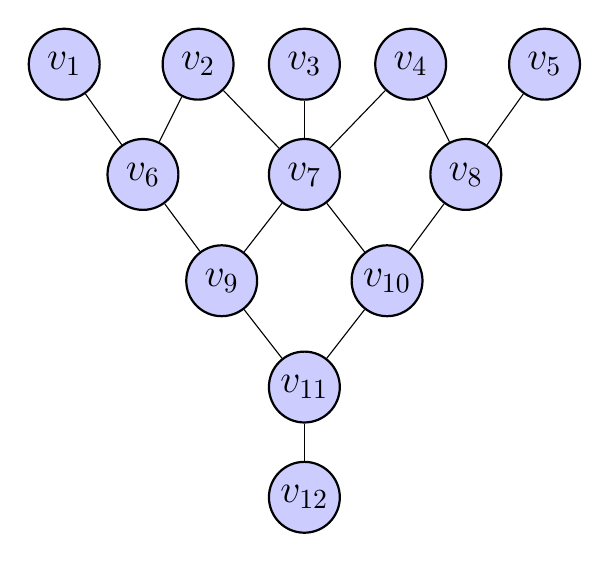
\begin{tikzpicture}[
  scale=1,
  vnode/.style={circle, fill=blue!20, draw=black, thick, minimum size=9mm, inner sep=0pt, font=\Large}
]
  % Vértices
  \node[vnode] (v1)  at (0.4, 5.5) {$v_1$};
  \node[vnode] (v2)  at (2.1, 5.5) {$v_2$};
  \node[vnode] (v3)  at (3.45, 5.5) {$v_3$};
  \node[vnode] (v4)  at (4.8, 5.5) {$v_4$};
  \node[vnode] (v5)  at (6.5, 5.5) {$v_5$};
  \node[vnode] (v6)  at (1.4, 4.1) {$v_6$};
  \node[vnode] (v7)  at (3.45, 4.1) {$v_7$};
  \node[vnode] (v8)  at (5.5, 4.1) {$v_8$};
  \node[vnode] (v9)  at (2.4, 2.75) {$v_9$};
  \node[vnode] (v10) at (4.5, 2.75) {$v_{10}$};
  \node[vnode] (v11) at (3.45, 1.4) {$v_{11}$};
  \node[vnode] (v12) at (3.45, 0) {$v_{12}$};

  % Aristas
  \foreach \from/\to in {v1/v6, v2/v6, v2/v7, v3/v7, v4/v7, v4/v8, v5/v8,
                         v6/v9, v7/v9, v7/v10, v8/v10, v9/v11, v10/v11, v11/v12}
    \draw (\from) -- (\to);
\end{tikzpicture}
}}}$
            &
            $\vcenter{\hbox{\tiny$\setcounter{MaxMatrixCols}{12}\begin{pmatrix}
         0 & 0 & 0 & 0 & 0 & 1 & 0 & 0 & 0 & 0 & 0 & 0 \\
         0 & 0 & 0 & 0 & 0 & 1 & 1 & 0 & 0 & 0 & 0 & 0 \\
         0 & 0 & 0 & 0 & 0 & 0 & 1 & 0 & 0 & 0 & 0 & 0 \\
         0 & 0 & 0 & 0 & 0 & 0 & 1 & 1 & 0 & 0 & 0 & 0 \\
         0 & 0 & 0 & 0 & 0 & 0 & 0 & 1 & 0 & 0 & 0 & 0 \\
         1 & 1 & 0 & 0 & 0 & 0 & 0 & 0 & 1 & 0 & 0 & 0 \\
         0 & 1 & 1 & 1 & 0 & 0 & 0 & 0 & 1 & 1 & 0 & 0 \\
         0 & 0 & 0 & 1 & 1 & 0 & 0 & 0 & 0 & 1 & 0 & 0 \\
         0 & 0 & 0 & 0 & 0 & 1 & 1 & 0 & 0 & 0 & 1 & 0 \\
         0 & 0 & 0 & 0 & 0 & 0 & 1 & 1 & 0 & 0 & 1 & 0 \\
         0 & 0 & 0 & 0 & 0 & 0 & 0 & 0 & 1 & 1 & 0 & 1 \\
         0 & 0 & 0 & 0 & 0 & 0 & 0 & 0 & 0 & 0 & 1 & 0
      \end{pmatrix}$}}$ \\
            \noalign{\vspace{6pt}}
         \end{tabular}%
      } \\
      \hline
      \multicolumn{3}{c}{\textbf{Topología de adyacencia}} \\
      \hline
      Abiertos subbásicos & Vecindades mínimas & Topología \\
      \hline
         ${A_{v_1}=\{v_6\}}$\par
         ${A_{v_2}=\{v_6,v_7\}}$\par
         ${A_{v_3}=\{v_7\}}$\par
         ${A_{v_4}=\{v_7,v_8\}}$\par
         ${A_{v_5}=\{v_8\}}$\par
         ${A_{v_6}=\{v_1,v_2,v_9\}}$\par
         ${A_{v_7}=\{v_2,v_3,v_4,v_9,v_{10}\}}$\par
         ${A_{v_8}=\{v_4,v_5,v_{10}\}}$\par
         ${A_{v_9}=\{v_6,v_7,v_{11}\}}$\par
         ${A_{v_{10}}=\{v_7,v_8,v_{11}\}}$\par
         ${A_{v_{11}}=\{v_9,v_{10},v_{12}\}}$\par
         ${A_{v_{12}}=\{v_{11}\}}$
      &
         ${U_{v_1}=\{v_1,v_2,v_9\}}$\par
         ${U_{v_2}=\{v_2,v_9\}}$\par
         ${U_{v_3}=\{v_2,v_3,v_4,v_9,v_{10}\}}$\par
         ${U_{v_4}=\{v_4,v_{10}\}}$\par
         ${U_{v_5}=\{v_4,v_5,v_{10}\}}$\par
         ${U_{v_6}=\{v_6\}}$\par
         ${U_{v_7}=\{v_7\}}$\par
         ${U_{v_8}=\{v_8\}}$\par
         ${U_{v_9}=\{v_9\}}$\par
         ${U_{v_{10}}=\{v_{10}\}}$\par
         ${U_{v_{11}}=\{v_{11}\}}$\par
         ${U_{v_{12}}=\{v_9,v_{10},v_{12}\}}$
      &
         No discreta, con 528 abiertos \\[6pt]
      \hline
      \multicolumn{3}{c}{\textbf{Topología de incidencia}} \\
      \hline
      Abiertos subbásicos & Vecindades mínimas & Topología \\
      \hline
         ${e_{1}=\{v_1,v_6\}}$\par
         ${e_{2}=\{v_2,v_6\}}$\par
         ${e_{3}=\{v_2,v_7\}}$\par
         ${e_{4}=\{v_3,v_7\}}$\par
         ${e_{5}=\{v_4,v_7\}}$\par
         ${e_{6}=\{v_4,v_8\}}$\par
         ${e_{7}=\{v_5,v_8\}}$\par
         ${e_{8}=\{v_6,v_9\}}$\par
         ${e_{9}=\{v_7,v_9\}}$\par
         ${e_{10}=\{v_7,v_{10}\}}$\par
         ${e_{11}=\{v_8,v_{10}\}}$\par
         ${e_{12}=\{v_9,v_{11}\}}$\par
         ${e_{13}=\{v_{10},v_{11}\}}$\par
         ${e_{14}=\{v_{11},v_{12}\}}$
      &
         ${U_{v_1}=\{v_1,v_6\}}$\par
         ${U_{v_2}=\{v_2\}}$\par
         ${U_{v_3}=\{v_3,v_7\}}$\par
         ${U_{v_4}=\{v_4\}}$\par
         ${U_{v_5}=\{v_5,v_8\}}$\par
         ${U_{v_6}=\{v_6\}}$\par
         ${U_{v_7}=\{v_7\}}$\par
         ${U_{v_8}=\{v_8\}}$\par
         ${U_{v_9}=\{v_9\}}$\par
         ${U_{v_{10}}=\{v_{10}\}}$\par
         ${U_{v_{11}}=\{v_{11}\}}$\par
         ${U_{v_{12}}=\{v_{11},v_{12}\}}$
      &
         No discreta, con 1296 abiertos \\[6pt]
      \hline
   \end{tabular}
   \caption{Topologías de adyacencia e incidencia de $G_6$}
   \label{tab:topologias_G_6}

   \vspace{1em}
   \begin{minipage}{\textwidth}
      \normalsize
      El grafo $G_6$ es un fragmento del \textit{Grafo de Young-Fibonacci}.
   \end{minipage}
\end{table}
